
\usepackage{amsmath,amssymb}
\usepackage{booktabs}
\usepackage{graphicx}
\usepackage{url}

\begin{document}

\title{Rollout-Aligned Uncertainty Learning for Probabilistic Battery State-of-Health Forecasting}

\author{
\IEEEauthorblockN{
Feng Ruiyang\IEEEauthorrefmark{1} and Supervisor Name\IEEEauthorrefmark{1}\IEEEauthorrefmark{2}
}
\IEEEauthorblockA{\IEEEauthorrefmark{1}
Department of Computing, City University of Hong Kong (Dong Guan)\\
Email: 72400082@cityu-dg.edu.cn}
\IEEEauthorblockA{\IEEEauthorrefmark{2}
Corresponding author: Supervisor Name, email: supervisor@example.com}
}

\maketitle

\begin{abstract}
Accurate long-horizon battery state-of-health (SoH) forecasting is important
for battery management systems because prediction errors and uncertainty can
accumulate over future cycles. This paper studies probabilistic SoH forecasting
under deployment-like autoregressive rollout. We use a Transformer-based
degradation model with a Variational Bayesian Last Layer (VBLL) output head and
compare teacher-forced training with a stochastic rollout-aligned objective.
The rollout-aligned objective feeds sampled predictions back into the decoder
during training and optimizes a sample-based Continuous Ranked Probability
Score (CRPS) together with a non-negativity penalty.

Experiments are conducted with cell-level splits and free-running stochastic
rollout evaluation. In per-cell macro evaluation on the main test split, the
rollout-aligned model reduces CRPS from 0.00539 to 0.00278 compared with the
teacher-forced CRPS-trained VBLL baseline. It also reduces the 90\% prediction
interval width from 0.05603 to 0.02014 while maintaining 90\% coverage at
0.95258. These results show that rollout-aligned training can improve
long-horizon probabilistic SoH forecasting without changing the model
architecture or uncertainty head.
\end{abstract}

\begin{IEEEkeywords}
Battery state of health, probabilistic forecasting, uncertainty estimation,
rollout training, Variational Bayesian Last Layer.
\end{IEEEkeywords}

\section{Introduction}

Lithium-ion batteries are widely used in electric vehicles, grid-scale energy
storage, consumer electronics, and aerospace systems because of their high
energy density and rechargeability. During repeated charge and discharge,
electrochemical aging mechanisms such as loss of lithium inventory, loss of
active material, impedance growth, and side reactions gradually reduce the
capacity-based state of health (SoH). If a battery management system (BMS)
cannot accurately monitor current SoH and anticipate future degradation, it
may make unsafe charging or discharging decisions, increasing the risk of
over-charge, over-discharge, thermal stress, and premature retirement.

Recent advances in data-driven methods have substantially improved battery SoH
estimation and forecasting. Severson et al.~\cite{severson2019} showed
that early-cycle discharge-voltage variance features can predict battery cycle
life before obvious capacity degradation. More recent Transformer-based and
self-attention models have moved from single-point SoH estimation toward
future degradation-trajectory prediction \cite{bellomo2025transformersoh,
huang2026ic2ml,hu2025batterygpt}. For uncertainty-aware prediction,
likelihood-based losses, Bayesian or ensemble models, evidential
distributions, and interval metrics have been used
\cite{munna2026fusion,parimala2026,wang2026uqreview}.

However, most uncertainty-aware SoH studies do not isolate the effect of
multi-step rollout training. Many sequence models are trained with teacher
forcing, where the decoder receives true previous SoH values, while deployment
requires feeding back the model's own predictions. This exposure-bias problem
\cite{bengio2015scheduled} can affect both point accuracy and predictive
uncertainty. This paper fills this gap by keeping the degradation encoder,
autoregressive decoder, and Variational Bayesian Last Layer (VBLL) uncertainty
head fixed, and comparing teacher-forced training with a stochastic rollout
objective for long-horizon probabilistic SoH forecasting.

The rest of this paper is organized as follows. Section~II reviews related
work on battery health forecasting, probabilistic uncertainty, and
autoregressive rollout. Section~III formulates the probabilistic multi-step
SoH forecasting problem. Section~IV describes the fixed model architecture and
rollout-aligned training objective. Section~V presents the experimental setup,
and Section~VI reports the results and discussion. Sections~VII and VIII
summarize limitations and conclusions, respectively.

\begin{figure*}[!t]
\centering
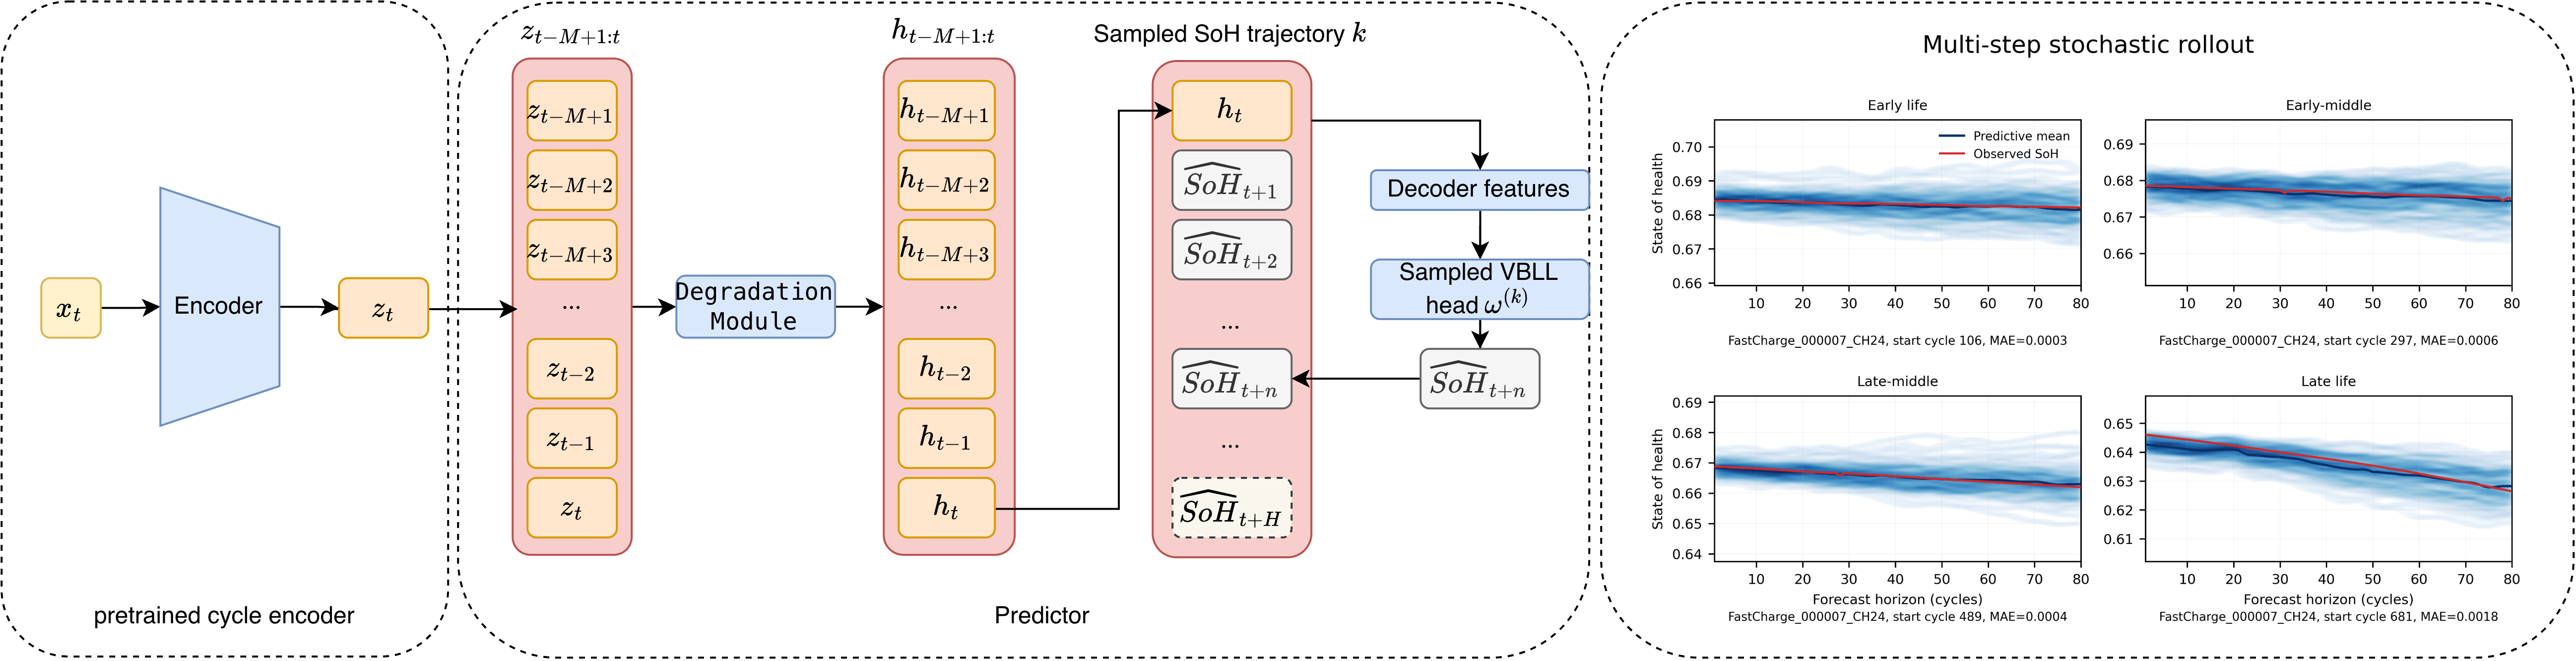
\includegraphics[width=\textwidth]{figures/rollout_framework.png}
\caption{Overview of the rollout-aligned probabilistic SoH forecasting
framework. A pretrained cycle encoder extracts latent cycle representations,
the degradation module aggregates the latent history, and the autoregressive
VBLL decoder generates stochastic future SoH trajectories. Representative
rollouts across different battery life stages are shown on the right.}
\label{fig:rollout-framework}
\end{figure*}

\section{Related Work}

\subsection{Battery Health Forecasting}

Battery health forecasting has progressed from feature-based early-life
prediction to sequence models for complete degradation trajectories. Severson
et al.~\cite{severson2019} showed that early-cycle discharge voltage can predict
battery cycle life before clear capacity degradation. Bellomo
et al.~\cite{bellomo2025transformersoh} and Huang et al.~\cite{huang2026ic2ml}
used Transformer-based representations for multi-step SoH and RUL prediction,
while BatteryGPT~\cite{hu2025batterygpt} and Lim and
See~\cite{lim2026worldmodel} modeled future evolution through autoregressive
charging-data or latent-dynamics rollouts. However, these studies mainly
provide deterministic forecasts or do not isolate teacher-forced from
stochastic rollout-aligned training under a common probabilistic head.

\subsection{Probabilistic Forecasting and Uncertainty}

Uncertainty-aware battery forecasting can use Gaussian likelihoods, Bayesian
neural networks, ensembles, Monte Carlo dropout, conformal prediction, or
last-layer Bayesian approximations. Recent SoH studies have used
distribution-free prediction intervals and probabilistic Transformer-based heads to
quantify uncertainty in health estimates
\cite{rasul2026ensemble,munna2026fusion}.
More broadly, uncertainty can be represented with Bayesian, ensemble,
evidential, interval, or other second-order methods
\cite{wang2026uqreview}. This paper uses a Variational Bayesian Last Layer
(VBLL), which places a variational posterior only on the final output layer
\cite{harrison2024vbll}. This choice gives stochastic forecast trajectories
with low extra cost, but it does not fully separate aleatoric and epistemic
uncertainty.

\subsection{Autoregressive Rollout}

Autoregressive multi-step prediction can be trained with teacher forcing or
evaluated under free rollout. For deployment, free rollout is the relevant
setting because the model must condition on its own earlier predictions.
Scheduled sampling reduces this training--inference gap by replacing some
ground-truth inputs with model predictions \cite{bengio2015scheduled}. Our
method extends this idea to probabilistic SoH forecasting by using sampled
free-running trajectories in the training loss. The evaluation focuses on
horizon-wise marginal calibration of sampled SoH forecasts rather than full
joint trajectory calibration.

\section{Problem Formulation}

For a given cell, let $x_t \in \mathbb{R}^{L \times C}$ be the measured cycle
sequence at cycle $t$, where $L$ is the resampled sequence length and $C$
denotes the voltage, current, and temperature channels when temperature is
available. Let $y_t$ be the SoH label. Cell indices are omitted when clear.
Given a history window of length $M$, the goal is to estimate the conditional
distribution
\begin{equation}
p\left(y_{t+1:t+H} \mid x_{t-M+1:t}, y_{t-M+1:t}, \mathcal{D}\right),
\end{equation}
where $H$ is the forecast horizon and $\mathcal{D}$ is the training set. A valid window is a
cell-level history--forecast window for which all required history cycles and
future SoH targets are observed and finite after preprocessing. The formal problem
assumes that future operating conditions are fixed by the dataset protocol or
implicitly represented by the observed history. It does not address arbitrary
future changes in charge protocol, ambient temperature, or load profile.

All splits are made at the cell level. This avoids leakage where cycles from
the same cell appear in both training and test sets. Future cycles that do not
exist for a short cell are masked, and losses and metrics are computed only on
finite valid targets.

\section{Method}

Figure~\ref{fig:rollout-framework} illustrates the inference pipeline. A
frozen pretrained encoder maps each measured cycle to a latent vector, and
consecutive latent vectors are aggregated by the Transformer-based degradation
module. The final degradation representation is then used by the
autoregressive VBLL decoder to generate stochastic future SoH trajectories.

\subsection{Cycle Representation}

A Transformer-based autoencoder compresses each normalized cycle curve into
a latent vector while preserving relevant cycle information:
\begin{equation}
z_t = E_{\phi}(x_t), \qquad z_t \in \mathbb{R}^{d_z}.
\end{equation}
Here, $E_{\phi}$ denotes the cycle encoder and $\phi$ denotes its model
parameters.
The latent dimension $d_z$ is fixed within each controlled comparison. The
autoencoder is trained with reconstruction mean squared error in the normalized
input space.

\subsection{Transformer-Based Degradation Module}

The degradation module is a causal history aggregator. Given the latent
window
\begin{equation}
Z_{t-M+1:t} = [z_{t-M+1}, \ldots, z_t],
\end{equation}
it produces a causal hidden-state sequence
\begin{equation}
H_{t-M+1:t}
=
[h_{t-M+1}, \ldots, h_t]
=
A_{\eta}(Z_{t-M+1:t}),
\end{equation}
and uses the last valid hidden state as the degradation state:
\begin{equation}
s_t = h_t .
\end{equation}
Here, $A_{\eta}$ denotes the Transformer-based degradation module and $\eta$
denotes its model parameters. In addition to the final degradation state used by
the SoH decoder, the history aggregator contains an auxiliary one-step latent
prediction head inside the observed history window:
\begin{equation}
\hat z_{i+1}=g_{\xi}(h_i),
\quad i=t-M+1,\ldots,t-1 .
\end{equation}
Here, $g_{\xi}$ is the auxiliary latent prediction head and $\xi$ denotes its
parameters, separate from the degradation-module parameters $\eta$. This head
predicts the one-step-shifted latent window $Z_{t-M+2:t}$ within the observed
history. It is used only as an auxiliary regularizer.
The auxiliary latent loss is
\begin{equation}
\mathcal{L}_{\mathrm{state}}
=
\frac{1}{|\Omega_z|}
\sum_{(b,i)\in\Omega_z}
\|\hat z_{b,i+1}-z_{b,i+1}\|_2^2,
\end{equation}
where $\Omega_z$ contains valid next-latent targets inside the observed history
window. Here, each $b$ corresponds to one length-$M$ history-window sample, and
$i$ indexes a position inside that window.

\subsection{VBLL SoH Decoder}

The SoH decoder is a two-layer autoregressive Transformer-based decoder. It
receives the degradation state $s_t$ as memory and previous SoH values as
decoder inputs. The output layer is a VBLL linear head. Its weights and bias are
modeled with a mean-field Gaussian posterior:
\begin{equation}
q(\omega)=\mathcal{N}(\mu_{\omega},\operatorname{diag}(\sigma_{\omega}^2)),
\qquad
p(\omega)=\mathcal{N}(0,\sigma_p^2 I).
\end{equation}
Here, $\omega$ denotes the VBLL output-layer parameters, $q(\omega)$ is their
learned variational posterior, and $p(\omega)$ is the zero-mean isotropic
Gaussian prior. The vectors $\mu_{\omega}$ and $\sigma_{\omega}$ denote the
posterior mean and standard deviation, while $\sigma_p$ is the prior standard
deviation. For trajectory $k$, one parameter sample is drawn as
$\omega^{(k)}=\mu_{\omega}+\sigma_{\omega}\odot\epsilon^{(k)}$, where
$\epsilon^{(k)}\sim\mathcal{N}(0,I)$, and is held fixed across all forecast
steps. Because no additional observation noise is sampled, the resulting
trajectory intervals reflect uncertainty from the VBLL output-layer posterior
rather than the full outcome predictive distribution. This gives free-running
posterior sample paths:
\begin{equation}
\hat{y}_{t+h}^{(k)} =
f_{\psi,\omega^{(k)}}(s_t, \hat{y}_{t+1:t+h-1}^{(k)}), \quad
\omega^{(k)} \sim q(\omega).
\end{equation}
Here, $f_{\psi,\omega^{(k)}}$ denotes the autoregressive SoH forecasting
function that maps the degradation state and the previously generated SoH
prefix to the next SoH prediction. The symbol $\psi$ denotes the deterministic parameters of the feature extractor and
autoregressive decoder excluding the sampled VBLL output-layer parameters,
$\omega^{(k)}$ denotes the independently sampled output-layer parameters for
the $k$th trajectory, and $\hat y_{t+h}^{(k)}$ is the resulting sampled SoH
prediction at horizon step $h$. Different trajectories use independent
posterior samples.
The rollout is initialized with the last observed SoH value $y_t$.

\subsection{Teacher-Forced Training}

In teacher-forced training, the decoder input at step $h$ is the true previous
SoH. The data-fit loss is the masked Gaussian negative log-likelihood:
\begin{equation}
\mathcal{L}_{\mathrm{NLL}}
=
\frac{1}{|\Omega|}
\sum_{(b,h)\in\Omega}
\frac{1}{2}
\left[
\frac{(y_{b,h}-\mu_{b,h})^2}{\sigma_{b,h}^2}
+ \log \sigma_{b,h}^2
\right].
\end{equation}
Here, $b$ has the same meaning as in the auxiliary latent loss: it indexes one
length-$M$ history-window sample. The index $h$ denotes the forecast horizon
step, and $\Omega$ contains valid window--horizon SoH targets.
The full teacher-forced objective is
\begin{equation}
\mathcal{L}_{\mathrm{TF}}
=
\mathcal{L}_{\mathrm{NLL}}
+ \lambda_{\mathrm{state}}\mathcal{L}_{\mathrm{state}}
+ \beta_{\mathrm{KL}}\mathrm{KL}(q(\omega)\|p(\omega)).
\end{equation}
The KL term is the Kullback--Leibler divergence from the learned VBLL posterior
$q(\omega)$ to the prior $p(\omega)$, and it regularizes the last-layer posterior
toward the prior. The coefficient $\beta_{\mathrm{KL}}$ controls the strength of
this variational regularization.
We use this as a $\beta$-weighted variational last-layer objective rather than
claiming a full Bayesian treatment of all network parameters.

\subsection{Rollout-Aligned Probabilistic Training}

Rollout-aligned training adds stochastic free-running trajectories to the
training objective. At each training window, the model samples $K$ trajectories
and feeds each sampled prediction back to the next step. Gradients are
propagated through the autoregressive rollout, allowing errors at later
forecast steps to update the earlier prediction steps on which they depend.
Scheduled sampling is also applied to the likelihood branch, where each
ground-truth decoder input is replaced by the posterior-mean prediction with
probability $p_{\mathrm{ss}}$. This probability increases linearly from 0 to
0.25 during training, gradually exposing the decoder to generated prefixes.
The main stochastic rollout loss is the empirical CRPS:
\begin{equation}
\widehat{\mathrm{CRPS}}
=
\frac{1}{K}\sum_{k=1}^{K} |\hat{y}^{(k)}-y|
-
\frac{1}{2K^2}\sum_{k=1}^{K}\sum_{j=1}^{K}
|\hat{y}^{(k)}-\hat{y}^{(j)}|.
\label{eq:empirical-crps}
\end{equation}
This sample form follows the proper scoring rule view of probabilistic
forecast evaluation \cite{gneiting2007scoring}. It is computed over valid
masked horizons. The current implementation uses $K=4$ training samples and
a horizon curriculum of 20, 40, and 80 steps. A
linear non-negativity penalty discourages negative SoH samples:
\begin{equation}
\mathcal{L}_{\mathrm{neg}}
=
\frac{1}{K|\Omega|}
\sum_{k=1}^{K}\sum_{(b,h)\in\Omega}
\max(0,-\hat{y}_{b,h}^{(k)}).
\end{equation}
The complete rollout-aligned objective is
\begin{equation}
\mathcal{L}_{\mathrm{rollout}}
=
\mathcal{L}_{\mathrm{TF}}
+ \lambda_{\mathrm{CRPS}}\mathcal{L}_{\mathrm{CRPS}}
+ \lambda_{\mathrm{neg}}\mathcal{L}_{\mathrm{neg}}.
\end{equation}
The non-negativity penalty is applied in the original SoH scale. It does not
guarantee monotonic degradation or hard physical consistency. It only reduces
invalid negative sampled SoH values.

\section{Experimental Setup}

\subsection{Data and Splits}

All models use the same cell-level split, pretrained cycle encoder, latent
representations, model size, and optimizer settings. Normalization statistics
are fitted on training cells only. Every model is evaluated by an 80-step
free-running rollout; probabilistic metrics use 128 posterior trajectories per
valid test window. Best checkpoints are selected exclusively on validation
data using each model's corresponding validation objective.

The main experiment uses a processed Severson-derived LFP fast-charge corpus
\cite{severson2019}. The cell-level split contains 98 training cells, 21
validation cells, and 21 test cells. After applying the 30-cycle history and
80-cycle forecast window, the test rollout evaluation contains 17,317 valid
windows from 20 test cells. The remaining test cell is excluded because it
contains fewer than $M+H$ cycles. Additional details on processed cycle counts, SoH
label construction, and the distinction from the original 124-cell subset are
given in Appendix~\ref{app:data-processing}.

\subsection{Compared Methods}

Table~\ref{tab:design} summarizes the controlled comparison. The key
identification step is the middle row: VBLL-TF-CRPS uses the same CRPS-related
training terms as VBLL-Rollout-CRPS but keeps teacher-forced prefixes. This
separates objective matching from generated-prefix training. All probabilistic
models share the same encoder, latent cache, VBLL head, and free-rollout
evaluation protocol. A deterministic teacher-forced model is reported as an
additional point-forecast baseline. It is not used to claim uncertainty
calibration. We also include VBLL-Rollout-CRPS-fair, which excludes self-pairs
from the finite-ensemble CRPS and replaces the $K^2$ pairwise normalization by
$K(K-1)$ while retaining generated-prefix rollout training. The main
hyperparameters are listed in Appendix
Table~\ref{tab:appendix-hparams}. In Table~\ref{tab:design}, ``Curr.'' denotes
rollout curriculum training; the fair-CRPS variant differs from
VBLL-Rollout-CRPS only in its finite-ensemble CRPS estimator.

\begin{table}[t]
\centering
\scriptsize
\caption{Training design.}
\label{tab:design}
\setlength{\tabcolsep}{2pt}
\begin{tabular}{@{}lcccc@{}}
\toprule
Method & Prefix & NLL & CRPS+Neg. & Curr. \\
\midrule
VBLL-TF-NLL & true & \checkmark & -- & -- \\
VBLL-TF-CRPS & true & \checkmark & \checkmark & \checkmark \\
VBLL-Rollout-CRPS & sampled & \checkmark & \checkmark & \checkmark \\
\bottomrule
\end{tabular}
\end{table}

\subsection{Metrics}

We report Mean Absolute Error (MAE), Root Mean Squared Error (RMSE), CRPS,
Prediction Interval Coverage Probability
(PICP), and Mean Prediction Interval Width (MPIW). Following the
calibration--sharpness view of probabilistic forecasts
\cite{gneiting2007calibration}, PICP is always interpreted together with
MPIW. A higher coverage is not necessarily better if it is obtained by overly
wide intervals. If the empirical coverage is far above the nominal level, we
report it as conservative uncertainty rather than as a calibration improvement.

For a nominal interval level $\alpha$, the PICP is
\begin{equation}
\mathrm{PICP}_{\alpha}
=
\frac{1}{|\Omega|}
\sum_{(b,h)\in\Omega}
\mathbb{I}\{y_{b,h} \in [l_{\alpha,b,h},u_{\alpha,b,h}]\},
\end{equation}
and the MPIW is
\begin{equation}
\mathrm{MPIW}_{\alpha}
=
\frac{1}{|\Omega|}
\sum_{(b,h)\in\Omega}
(u_{\alpha,b,h}-l_{\alpha,b,h}).
\end{equation}
Here, $l_{\alpha,b,h}$ and $u_{\alpha,b,h}$ are the lower and upper bounds of
the nominal $\alpha$ prediction interval for window--horizon pair $(b,h)$.
The indicator function $\mathbb{I}\{\cdot\}$ equals one when the true SoH
$y_{b,h}$ falls inside this interval and zero otherwise.
The intervals are central equal-tailed empirical quantile intervals from
$K_{\mathrm{eval}}=128$ stochastic rollout samples. We report horizon-wise
results at representative forecast steps. We additionally report per-cell
macro averages to prevent cells with more valid rollout windows from
dominating the aggregate evaluation.

\section{Results and Discussion}

\subsection{Overall Long-Horizon Forecasting}

Table~\ref{tab:overall} reports window-level free-running rollout performance
on the test split. Deterministic-TF is a point-forecast baseline, so
probabilistic metrics are not applicable. Probabilistic rows use 128 stochastic
rollout samples.

\begin{table}[t]
\centering
\scriptsize
\caption{Overall test performance.}
\label{tab:overall}
\setlength{\tabcolsep}{3pt}
\begin{tabular}{@{}lccccc@{}}
\toprule
Method & MAE & RMSE & CRPS & 90\% PICP & 90\% MPIW \\
\midrule
Deterministic-TF & 0.00750 & 0.01671 & -- & -- & -- \\
VBLL-TF-NLL & 0.00458 & 0.01658 & 0.00429 & 0.99912 & 0.04670 \\
VBLL-TF-CRPS & 0.00317 & 0.01597 & 0.00416 & 0.99918 & 0.04914 \\
VBLL-Rollout-CRPS & 0.00373 & 0.01530 & 0.00281 & 0.96342 & 0.02088 \\
VBLL-Rollout-CRPS-fair & 0.00258 & 0.01465 & 0.00197 & 0.77205 & 0.00836 \\
\bottomrule
\end{tabular}
\end{table}

\begin{table*}[t]
\centering
\scriptsize
\caption{Per-cell macro performance.}
\label{tab:cell-macro}
\setlength{\tabcolsep}{3pt}
\begin{tabular}{@{}lccccc@{}}
\toprule
Method & MAE & RMSE & CRPS & 90\% PICP & 90\% MPIW \\
\midrule
Deterministic-TF
& 0.00768 [0.00683, 0.00856]
& 0.01526 [0.01265, 0.01799]
& -- & -- & -- \\
VBLL-TF-NLL
& 0.00469 [0.00363, 0.00591]
& 0.01455 [0.01124, 0.01793]
& 0.00443 [0.00408, 0.00483]
& 0.99896 [0.99839, 0.99944]
& 0.04912 [0.04621, 0.05243] \\
VBLL-TF-CRPS
& 0.00625 [0.00556, 0.00694]
& 0.01571 [0.01265, 0.01869]
& 0.00539 [0.00505, 0.00572]
& 0.99698 [0.99327, 0.99941]
& 0.05603 [0.05390, 0.05806] \\
VBLL-Rollout-CRPS
& 0.00373 [0.00321, 0.00422]
& 0.01265 [0.00921, 0.01609]
& 0.00278 [0.00243, 0.00312]
& 0.95258 [0.90893, 0.98286]
& 0.02014 [0.01727, 0.02309] \\
VBLL-Rollout-CRPS-fair
& 0.00254 [0.00214, 0.00297]
& 0.01161 [0.00809, 0.01512]
& 0.00195 [0.00163, 0.00229]
& 0.74501 [0.67040, 0.81517]
& 0.00778 [0.00614, 0.00956] \\
\bottomrule
\end{tabular}
\end{table*}

The overall tables show the same main pattern: rollout-aligned training
improves the proper score and substantially tightens prediction intervals
relative to teacher-forced VBLL training.
Table~\ref{tab:cell-macro} reports per-cell macro results with 95\% bootstrap
confidence intervals. Each metric is first computed separately for each test
cell and then averaged across cells, so every cell receives equal weight
regardless of its number of valid rollout windows. Values in square brackets
denote 95\% confidence intervals obtained by bootstrap resampling over test
cells. The macro table is therefore the main statistical comparison. The
deterministic teacher-forced baseline gives a macro MAE of 0.00768. Adding the
VBLL probabilistic head and teacher-forced NLL training reduces macro MAE to
0.00469, but its prediction intervals are highly conservative, with 90\% PICP
of 0.99896.

The empirical-CRPS rollout model improves all three macro error scores relative
to the teacher-forced VBLL models. Compared with VBLL-TF-NLL, it reduces macro
MAE from 0.00469 to 0.00373 and CRPS from 0.00443 to 0.00278. Its 90\% PICP is
0.95258 with an MPIW of 0.02014, giving substantially sharper intervals than
the teacher-forced alternatives while remaining above the nominal coverage
level.

The fair-CRPS rollout control further reduces window-level MAE from 0.00373 to
0.00258 and CRPS from 0.00281 to 0.00197. However, its 90\% MPIW contracts from
0.02088 to 0.00836 while PICP falls from 0.96342 to 0.77205. Its cell-macro
PICP is 0.74501, and 17 of the 20 test cells fall below 0.90. The fair estimator
corrects the finite-ensemble self-pair bias but does not enforce interval
coverage; with only four training trajectories and uncertainty restricted to
the VBLL output layer, the resulting posterior trajectories are overly
concentrated. The lower CRPS therefore comes with systematic under-coverage
and overconfidence rather than uniformly better uncertainty quantification.

The aggregate sampled negative-SoH rate is below the displayed precision for
all VBLL rows, suggesting that the soft non-negativity penalty is effective in
this setting but not proving a hard physical constraint.

\subsection{Seed Robustness}

To assess sensitivity to predictor initialization, we evaluate
VBLL-Rollout-CRPS with the encoder and split seeds fixed at 42 and predictor
seeds 42, 8209, and 9181. Table~\ref{tab:seed-robustness} reports the results.

\begin{table}[t]
\centering
\scriptsize
\caption{Predictor-seed robustness.}
\label{tab:seed-robustness}
\setlength{\tabcolsep}{2pt}
\begin{tabular}{@{}ccccc@{}}
\toprule
Pred. seed & MAE & CRPS & 90\% PICP & 90\% MPIW \\
\midrule
42 & 0.00373 & 0.00281 & 0.96342 & 0.02088 \\
8209 & 0.00365 & 0.00274 & 0.98066 & 0.02437 \\
9181 & 0.00370 & 0.00296 & 0.99906 & 0.02740 \\
\bottomrule
\end{tabular}
\end{table}

\subsection{Horizon-Wise Behavior}

Table~\ref{tab:horizon} reports probabilistic forecasting results at
representative forecast steps.

\begin{table}[t]
\centering
\scriptsize
\caption{Horizon-wise results.}
\label{tab:horizon}
\setlength{\tabcolsep}{2pt}
\begin{tabular}{@{}llcccc@{}}
\toprule
Method & Horizon & MAE & CRPS & 90\% PICP & 90\% MPIW \\
\midrule
VBLL-TF-NLL & 1 & 0.00142 & 0.00128 & 0.99729 & 0.01131 \\
VBLL-TF-NLL & 20 & 0.00240 & 0.00263 & 0.99906 & 0.02785 \\
VBLL-TF-NLL & 50 & 0.00545 & 0.00508 & 0.99927 & 0.05694 \\
VBLL-TF-NLL & 80 & 0.00884 & 0.00743 & 0.99924 & 0.07900 \\
\midrule
VBLL-TF-CRPS & 1 & 0.00119 & 0.00123 & 0.99873 & 0.01171 \\
VBLL-TF-CRPS & 20 & 0.00257 & 0.00277 & 0.99923 & 0.03162 \\
VBLL-TF-CRPS & 50 & 0.00362 & 0.00487 & 0.99920 & 0.05782 \\
VBLL-TF-CRPS & 80 & 0.00456 & 0.00698 & 0.99924 & 0.08496 \\
\midrule
VBLL-Rollout-CRPS & 1 & 0.00329 & 0.00267 & 0.87671 & 0.01789 \\
VBLL-Rollout-CRPS & 20 & 0.00263 & 0.00213 & 0.98855 & 0.01878 \\
VBLL-Rollout-CRPS & 50 & 0.00418 & 0.00302 & 0.97203 & 0.02273 \\
VBLL-Rollout-CRPS & 80 & 0.00504 & 0.00374 & 0.94592 & 0.02334 \\
\bottomrule
\end{tabular}
\end{table}

\subsection{Discussion}

The main question is whether the improvement comes from matching the
probabilistic scoring rule or from exposing the model to generated prefixes
during training. The VBLL-TF-CRPS baseline already uses the same CRPS-related
loss terms as the rollout-aligned model, but it still conditions on true
prefixes. In Table~\ref{tab:overall}, VBLL-TF-CRPS only slightly improves over
VBLL-TF-NLL in CRPS, while both models remain conservative. In contrast,
VBLL-Rollout-CRPS improves CRPS and reduces interval width. This separation
supports the view that generated-prefix training is important for
probabilistic free rollout, not only the use of a CRPS-related loss.

The horizon-wise results show different uncertainty behavior. The two
teacher-forced VBLL models keep very high 90\% coverage at all reported
horizons, but their interval width grows strongly with horizon. For example,
VBLL-TF-CRPS increases from 0.01171 at horizon 1 to 0.08496 at horizon 80.
The rollout-aligned model has a much smaller width at horizon 80, 0.02334,
while keeping coverage at 0.94592. It is under-covered at horizon 1
(0.87671), which indicates that the method is not perfectly calibrated at all
horizons. However, the long-horizon behavior is sharper and closer to the
nominal coverage level than the teacher-forced alternatives.

Across predictor seeds 42, 8209, and 9181, MAE remains within
0.00365--0.00373 and CRPS within 0.00274--0.00296, indicating stable point
accuracy and probabilistic scoring performance. However, 90\% PICP varies from
0.96342 to 0.99906 and MPIW from 0.02088 to 0.02740, showing greater seed
sensitivity in interval calibration and sharpness. Because the encoder and
split seeds are fixed at 42, these results do not establish robustness to
encoder initialization or dataset partitioning.

The reported CRPS and PICP are computed step by step over horizons. They
measure horizon-wise marginal forecast quality and do not prove full joint
trajectory calibration. A multivariate score such as the Energy Score would be
needed to make a stronger claim about the complete joint distribution of
trajectories.

\section{Limitations}

Several limitations of this work should be noted. First, because we use a VBLL
head, only the final output layer is Bayesian; all remaining layers are
deterministic. Consequently, the
predictive uncertainty does not fully disentangle epistemic uncertainty from
aleatoric uncertainty. Second, the CRPS is computed using a finite ensemble of
rollout samples. When $K$ is small, the empirical CRPS is not a fair and
unbiased estimate of the score for the true underlying continuous predictive
distribution. Finally, evaluation is limited to a single processed
Severson-derived dataset. We leave common horizon cohorts and multivariate
trajectory calibration metrics for future work.

\section{Conclusion}

This work makes three main contributions. First, we propose a rollout-aligned
probabilistic framework for long-horizon battery SoH forecasting, representing
future degradation as multiple autoregressively generated stochastic
trajectories rather than isolated point estimates. Second, we develop a
stochastic rollout training strategy that feeds sampled SoH predictions back
into the decoder and directly optimizes the resulting multi-step forecasts
using sample-based CRPS. By training on its own generated prefixes, the model
reduces the mismatch between teacher-forced training and autoregressive
deployment. Third, experiments show that the proposed approach achieves the
best per-cell macro MAE, RMSE, and CRPS while producing substantially narrower
prediction intervals with coverage close to the nominal level. Its
effectiveness is further supported by horizon-wise evaluation and seed
robustness experiments. The current evidence is limited to horizon-wise
marginal calibration on one main cell-level split, so broader datasets and
joint trajectory scores remain future work.

\appendices

\section{Reproducibility Notes}

\subsection{Rollout-Aligned Training Algorithm}

Algorithm~\ref{alg:rollout-training} summarizes the main training procedure.
It is written at the level of the implemented data flow rather than as a new
optimization algorithm.

\begin{table}[h]
\centering
\scriptsize
\caption{Rollout-aligned probabilistic SoH training.}
\label{alg:rollout-training}
\begin{tabular}{@{}p{0.97\linewidth}@{}}
\toprule
\textbf{Input:} cycle sequences, SoH trajectories, trained cycle encoder
$f_\theta$, Transformer-based degradation module $g_\eta$, autoregressive decoder
$d_\psi$, VBLL last layer $q_\phi(\omega)$, horizon $H$, sample count $K$. \\
\midrule
1. Encode each observed cycle curve into a latent vector
$z_i=f_\theta(x_i)$. \\
2. Form a history window from the most recent $M$ latent vectors and observed
SoH values. \\
3. Compute the degradation state $s_t=g_\eta(z_{t-M+1:t})$. \\
4. Compute the teacher-forced VBLL negative log-likelihood and auxiliary
next-latent loss on valid training targets. \\
5. Draw $K$ VBLL output-layer samples and autoregressively generate $K$ SoH
trajectories for $H$ future cycles. At each rollout step, feed the sampled
prediction back to the decoder prefix. \\
6. Compute empirical CRPS over valid future targets and apply the soft
non-negativity penalty to sampled SoH values below zero. \\
7. Update model parameters with the weighted sum of teacher-forced NLL,
state loss, KL regularization, stochastic CRPS, and non-negativity loss. \\
\bottomrule
\end{tabular}
\end{table}

\subsection{CRPS Estimator}

For a scalar target $y$ and a predictive cumulative distribution function
$F$, the Continuous Ranked Probability Score can be written as
\begin{equation}
\mathrm{CRPS}(F,y)
=
\int_{-\infty}^{\infty}
\left(F(u)-\mathbf{1}\{y\le u\}\right)^2du .
\end{equation}
For an ensemble forecast with samples $\{\hat y^{(k)}\}_{k=1}^{K}$, the
integral definition is equivalent to the expectation identity
\begin{equation}
\mathrm{CRPS}(F,y)
=
\mathbb{E}_{X\sim F}|X-y|
-
\frac{1}{2}\mathbb{E}_{X,X'\sim F}|X-X'|.
\end{equation}
Replacing the two expectations by Monte Carlo averages gives the implemented
empirical estimator:
\begin{equation*}
\widehat{\mathrm{CRPS}}
=
\frac{1}{K}\sum_{k=1}^{K}|\hat y^{(k)}-y|
-
\frac{1}{2K^2}\sum_{k=1}^{K}\sum_{j=1}^{K}
|\hat y^{(k)}-\hat y^{(j)}|.
\end{equation*}
The first term rewards samples close to the observed target. The second term
rewards ensemble spread, so the score does not collapse to a deterministic
absolute-error objective. In the current implementation this score is computed
for each valid horizon and then averaged over the valid window--horizon
positions. A fair-ensemble variant excludes self-pairs and replaces $K^2$
with $K(K-1)$.

\subsection{Main Hyperparameters}

Table~\ref{tab:appendix-hparams} records the main hyperparameters used by the
scaled Severson experiments. The seed robustness runs keep the encoder and
split seeds fixed at 42 and change only the predictor seed.

\begin{table}[h]
\centering
\scriptsize
\caption{Main hyperparameters and reproducibility fields.}
\label{tab:appendix-hparams}
\setlength{\tabcolsep}{2pt}
\begin{tabular}{@{}p{0.40\columnwidth}p{0.53\columnwidth}@{}}
\toprule
Item & Value \\
\midrule
History window $M$ & 30 cycles \\
Forecast horizon $H$ & 80 cycles \\
Evaluation samples $K_{\mathrm{eval}}$ & 128 \\
Cycle encoder input & voltage, current, temperature \\
Cycle encoder & $d_z=256$, $d_{\mathrm{model}}=256$, 3 layers, 8 heads \\
Encoder training & batch 256, AdamW, lr $2.0{\times}10^{-4}$, weight decay
$1.0{\times}10^{-5}$ \\
Encoder scheduler & ReduceLROnPlateau, factor 0.5, patience 6, min lr
$1.0{\times}10^{-6}$; early stopping patience 12 \\
Degradation module & 2 layers, hidden dimension 512 \\
Autoregressive decoder & 2 layers, hidden dimension 512 \\
VBLL prior variance & 0.5 \\
Predictor optimizer & AdamW, base lr $2.0{\times}10^{-4}$, VBLL $\rho$ lr
$1.0{\times}10^{-3}$, weight decay $1.0{\times}10^{-5}$ \\
KL weight $\beta_{\mathrm{KL}}$ & $1.0{\times}10^{-4}$ \\
State-loss weight $\lambda_{\mathrm{state}}$ & 1.0 \\
CRPS weight $\lambda_{\mathrm{CRPS}}$ & 0.1 \\
Negative-SoH penalty $\lambda_{\mathrm{neg}}$ & 0.1 for stochastic rollout;
0 otherwise \\
Training rollout samples & $K=4$ \\
Rollout curriculum & 20, 40, and 80 steps from epochs 10, 30, and 50 \\
Scheduled sampling & probability linearly increases from 0 to 0.25 over 100
epochs for rollout-aligned runs \\
Main seeds & encoder 42, predictor 42 \\
Robustness seeds & encoder/split 42; predictor 42, 8209, and 9181 \\
\bottomrule
\end{tabular}
\end{table}

\subsection{Data Processing and Code Links}
\label{app:data-processing}

The processed LFP fast-charge corpus is derived from Severson
et al.~\cite{severson2019}. The split used in the main experiments contains
80,803 training cycles, 15,593 validation cycles, and 17,918 test cycles in
the processed tables. The SoH label is computed as discharge capacity divided
by the first positive finite discharge capacity of the same cell. The
processed dataset contains more cells than the 124-cell subset emphasized in
the original Severson et al. paper because the parser includes available
fast-charge processed cells from the local processed corpus. We therefore
report this as a processed Severson-derived corpus rather than as the exact
124-cell subset.

The final camera-ready version will provide a public GitHub repository
containing the code, processed-data manifest, configuration files, and
evaluation outputs: [TODO: GitHub repository URL].
The processed data release will document the original data source, parser
version, split file, channel normalization statistics, and checksum for each
artifact. The release will not replace the license or citation requirements
of the original battery datasets.

\bibliographystyle{IEEEtran}
\begin{thebibliography}{1}

\bibitem{su2024sohreview}
L.~Su, J.~Zhang, C.~Wang, Y.~Zhang, Z.~Li, Y.~Song, T.~Jin, and Z.~Dong,
``State-of-health estimation of lithium-ion batteries: A comprehensive
literature review from cell to pack levels,'' \emph{Energy Conversion and
Economics}, vol.~5, no.~3, pp. 166--188, 2024.

\bibitem{severson2019}
K.~A. Severson, P.~M. Attia, N.~Jin, N.~Perkins, B.~Jiang, Z.~Yang,
M.~H. Chen, M.~Aykol, P.~K. Herring, D.~Fraggedakis, M.~Z. Bazant,
S.~J. Harris, W.~C. Chueh, and R.~D. Braatz, ``Data-driven prediction of
battery cycle life before capacity degradation,'' \emph{Nature Energy},
vol.~4, pp. 383--391, 2019.

\bibitem{bellomo2025transformersoh}
M.~Bellomo, A.~Dolara, and F.~Grimaccia, ``An innovative Transformer-based
approach for state of health trajectory prediction and remaining useful life
estimation in lithium-ion batteries,'' in \emph{Proc. 2025 International
Conference on Clean Electrical Power (ICCEP)}, 2025,
doi: 10.1109/ICCEP65222.2025.11143638.

\bibitem{huang2026ic2ml}
X.~Huang, C.~Liang, S.~Tao, Y.~Che, N.~Bian, J.~Zhang, R.~Wang, Y.~Zhang,
B.~Xia, and X.~Zhang, ``IC2ML: Unified battery state-of-health, degradation
trajectory and remaining useful life prediction via intra-cycle and inter-cycle
enhanced machine learning,'' \emph{Journal of Power Sources}, vol.~666,
article 239148, 2026.

\bibitem{hu2025batterygpt}
J.~Hu, P.~Fu, Z.~Wei, Y.~Huang, J.~Early, A.~Fly, and Y.~Zhang, ``Early
prediction of lithium-ion battery degradation with a generative pre-trained
transformer,'' \emph{Nature Communications}, vol.~17, article 126, 2026.

\bibitem{munna2026fusion}
M.~A. Munna, Z.~Deng, J.~Wang, Z.~Yuan, F.~Zhang, and J.~Liu,
``Fusion-enhanced Transformer architecture for uncertainty-aware
state-of-health estimation of lithium-ion batteries using partial-voltage
data,'' \emph{Journal of Energy Storage}, vol.~164, article 122170, 2026.

\bibitem{parimala2026}
C.~H. Parimala, P.~S. Varma, R.~S. Kumar, A.~R. Singh,
B.~Mohapatra, and H.~K. Addis, ``Uncertainty aware hybrid learning framework
for fast and safe charging of lithium-ion batteries using multi-fidelity
observers,'' \emph{Scientific Reports}, vol.~16, article 2452, 2026.

\bibitem{wang2026uqreview}
K.~Wang, F.~Cuzzolin, K.~Shariatmadar, D.~Moens, and H.~Hallez,
``A review of uncertainty representation and quantification in neural
networks,'' \emph{IEEE Transactions on Pattern Analysis and Machine
Intelligence}, vol.~48, no.~3, pp. 2476--2495, 2026.

\bibitem{bengio2015scheduled}
S.~Bengio, O.~Vinyals, N.~Jaitly, and N.~Shazeer, ``Scheduled sampling for
sequence prediction with recurrent neural networks,'' in \emph{Advances in
Neural Information Processing Systems}, vol.~28, pp. 1171--1179, 2015.

\bibitem{lim2026worldmodel}
K.~C. Lim and K.~W. See, ``World model for battery degradation prediction under
non-stationary aging,'' arXiv:2603.10527, 2026.

\bibitem{rasul2026ensemble}
M.~J.~M.~A. Rasul, A.~Abbas, J.~Baek, and J.~Kim, ``A hybrid ensemble learning
framework with uncertainty quantification for state-of-health estimation in
lithium-ion batteries,'' \emph{Measurement}, vol.~266, article 120528, 2026.

\bibitem{harrison2024vbll}
J.~Harrison, J.~Willes, and J.~Snoek, ``Variational Bayesian last layers,'' in
\emph{International Conference on Learning Representations}, 2024.

\bibitem{gneiting2007scoring}
T.~Gneiting and A.~E. Raftery, ``Strictly proper scoring rules, prediction,
and estimation,'' \emph{Journal of the American Statistical Association},
vol.~102, no.~477, pp. 359--378, 2007.

\bibitem{gneiting2007calibration}
T.~Gneiting, F.~Balabdaoui, and A.~E. Raftery, ``Probabilistic forecasts,
calibration and sharpness,'' \emph{Journal of the Royal Statistical Society:
Series B (Statistical Methodology)}, vol.~69, no.~2, pp. 243--268, 2007.
\end{thebibliography}

\end{document}
